\chapter{RSCP-iBGP系统的设计实现}
\label{cha:design}

\section{本章引言}
本文基于软件路由器Quagga\cite{quagga}的开源代码,实现了RSCP-iBGP内部域间路由协议系统。该系统主要分三部分:边界路由器Route-Client、集中式的路由控制平台上运行的Route-Server、边界路由器与Route-Server之间的扩展iBGP通信协议。本章首先解释设计实现平台Quagga的概念以及其虚拟软件路由器上BGP的路由功能实现细节,之后详细介绍RSCP-iBGP系统的三个部分边界路由器、路由控制平台、通信接口的具体设计与实现。

\section{设计实现平台Quagga介绍}

\begin{figure}
  \centering
  % Requires \usepackage{graphicx}
  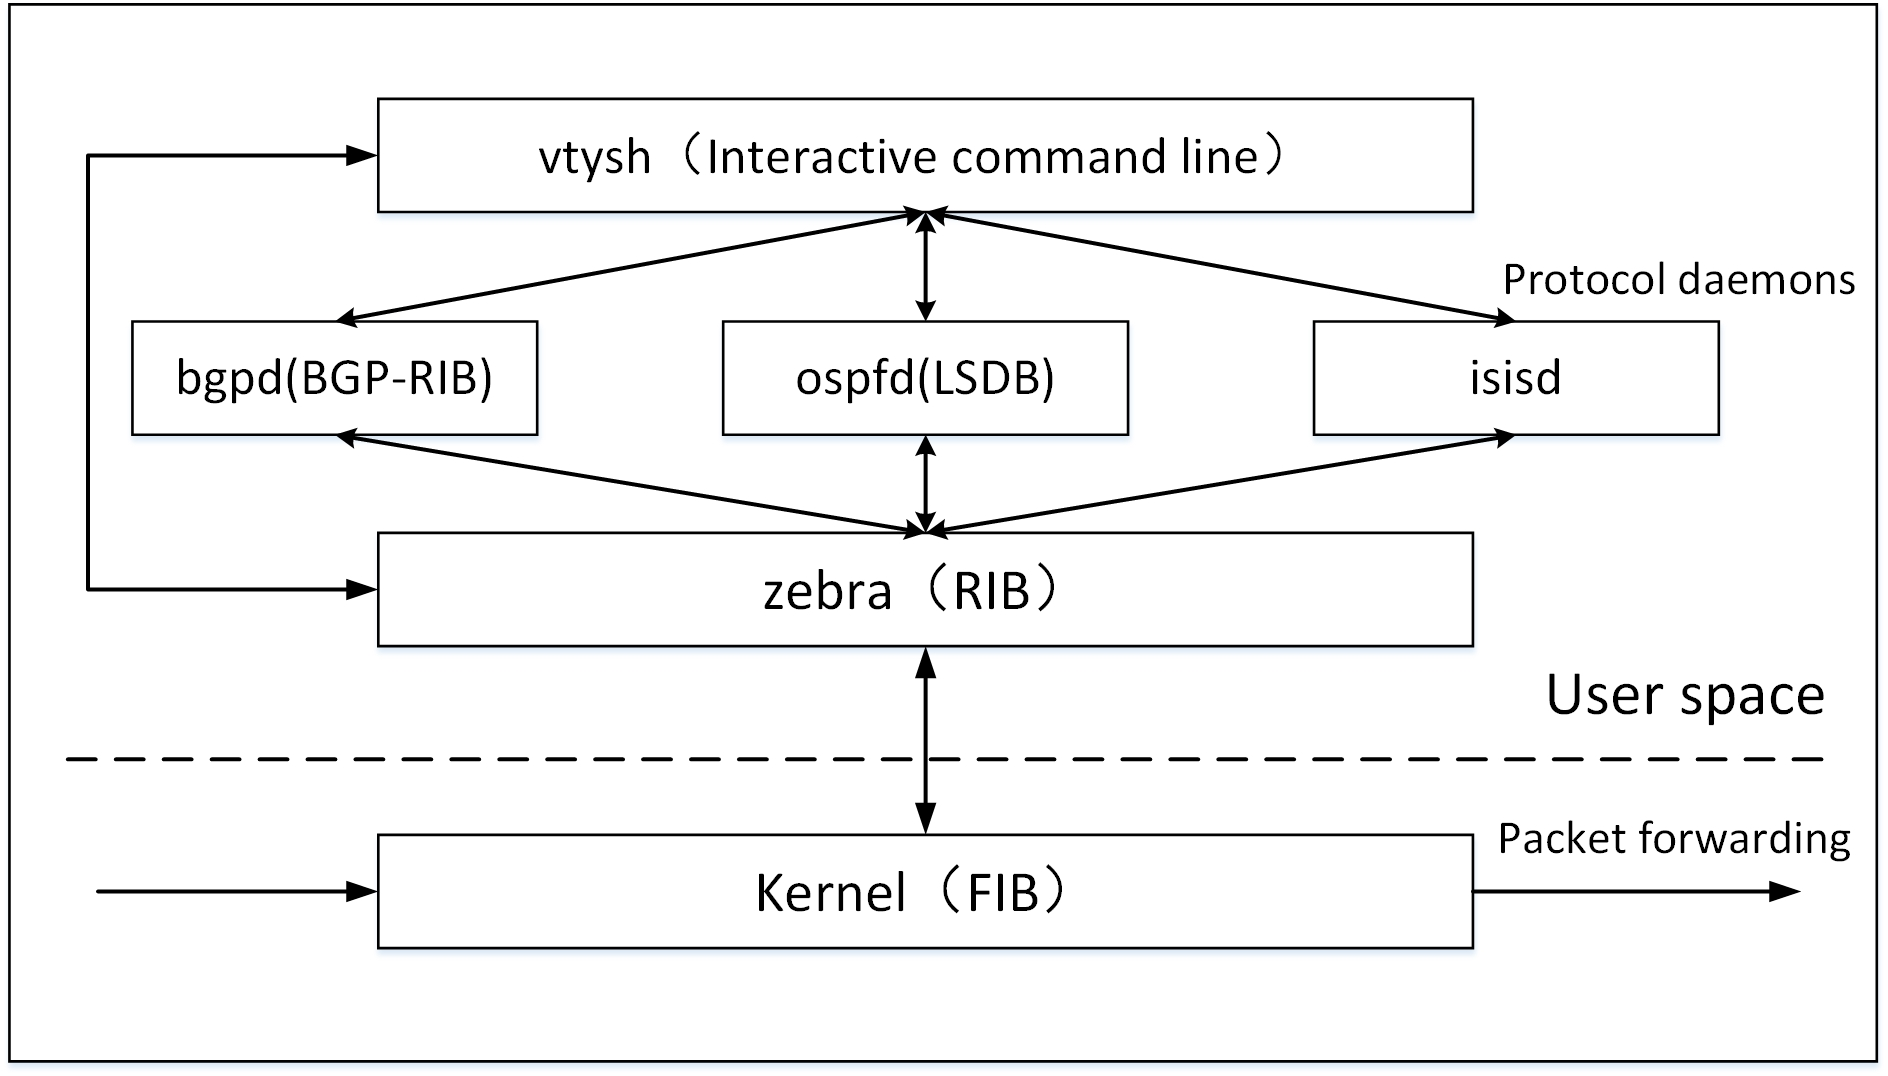
\includegraphics[width=0.75\textwidth]{quagga}
  \caption{Quagga系统结构图\cite{jakma2014quagga}}
  \label{fig:quagga}
\end{figure}


\subsection{基本概念及系统结构}
Quagga是一个比较成熟的虚拟路由器系统,该系统实现了多种网络协议,比如RIPv1、RIPv2、RIPng、OSPFv2、OSPFv3、BGPv4+、IS-IS等。Quagga中不同的网络协议需要运行不同的进程,属于多进程结构,协议之间相互独立,其本身的扩展性、维护性较强 \cite{quaggaThesis}。此外,Quagga中包含一个路由信息管理进程zebra,该进程和各种运行网络协议的进程通过ZServ协议进行交互,将运行网络协议进程产生的有效路由信息安装到内核\cite{jakma2014quagga}。每个协议进程均有自己的配置文件和终端接口,配置不同的网络需要在不同的网络进程内的配置文件中完成,非常麻烦。比如配置BGP网络时,需要在bgpd进程中的配置文件中完成;配置静态路由时,需要在zebra进程中的配置文件中完成。为此,Quagga存增设vtysh进程来对Quagga中的其他进程进行配置。vtysh提供一个交互式的命令行接口来输入配置信息,其和其他进程通信通过一个简单的字符串传输协议传输配置信息。在vtysh进程中可以完成针对其他网络协议的配置、静态路由等配置操作。Quagga的结构如图\ref{fig:quagga}。
\subsection{BGP协议的路由存储}

BGP协议中路由信息表有3种Adj-RIBs-In、Loc-RIB、Adj-RIBs-Out,Quagga中BGP协议的实现在bgpd进程中。bgpd进程中所有的数据结构均存储在bgp\_master结构体中,bgp\_master的成员变量中存在一个链表,包含了所有的bgp实例。每个bgp实例中存储了该BGP session的配置文件、一个包含所有的peer实例的链表、静态路由表、路由表(Loc-RIB,结构体为bgp\_table)等信息。


\begin{figure}
  \centering
  % Requires \usepackage{graphicx}
  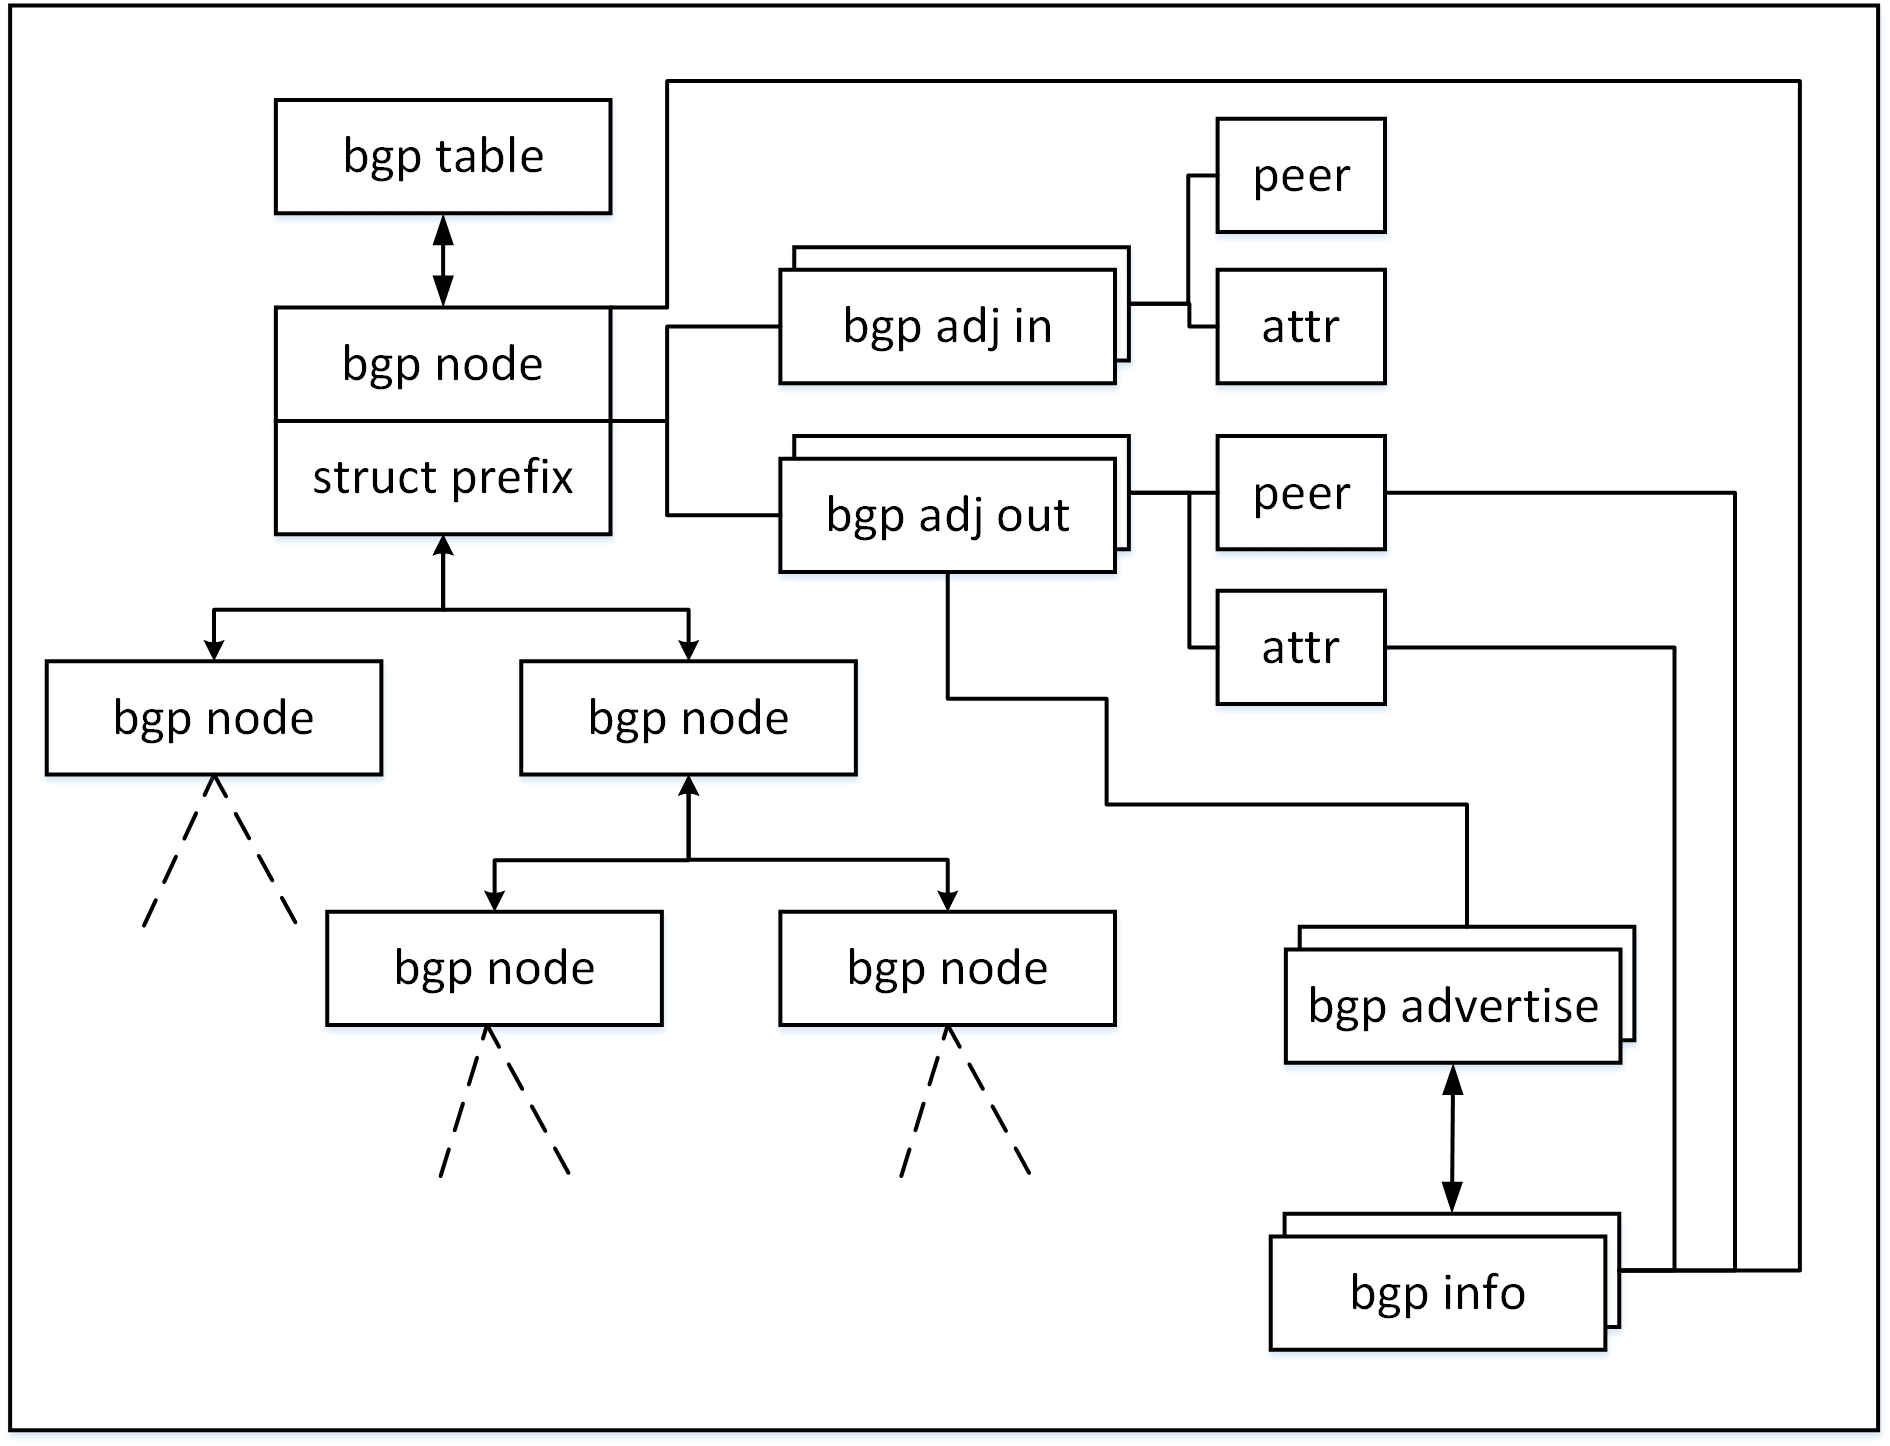
\includegraphics[width=0.75\textwidth]{storage}
  \caption{Quagga-bgpd:BGP路由表概括图\cite{jakma2014quagga}}
  \label{fig:storage}
\end{figure}

Quagga中路由表的存储使用radix二叉树\cite{quaggaThesis}存储结构,radix树是以二进制表示的键值作为树的节点,每个节点通过比较比特位来进行查找,radix二叉搜索树适合处理非常长的,可变长度的键值。每张Loc-RIB表存储在bgp\_table的结构体中,bgp\_table结构体有一个成员变量为bgp\_node类的结构体指针,该结构体指针是该Loc-RIB表radix树结构的根节点,所有路由表项的查找、删除等操作都从该根节点开始。bgp\_node结构体的实例代表的是某前缀所有的路由信息(每一条路由信息用bgp\_info结构体对应的实例表示),bgp\_node结构体中也存在指向bgp\_adj\_in和bgp\_adj\_out的指针。路由信息在bgp\_adj\_in和bgp\_adj\_out中的主要体现是通过他们的成员变量peer和attr。

当运行Quagga的虚拟路由器收到路由更新时,如果开启了Adj-RIBs-In存储设置,则会先根据前缀找到对应的bgp\_node,之后根据bgp\_node找到对应的adj\_rib\_in,对其进行更新。当BGP控制台需要输出某对等体的Adj-RIB-In表,则遍历所有的bgp\_node节点,根据bgp\_node找到每条前缀对应的adj\_rib\_in表,遍历该adj\_rib\_in表,如果某路由信息从该对等体收到的,则输出对应的路由信息。

针对某条路由信息bgp\_info向外进行路由宣告时,如果开启了Adj-RIBs-Out存储设置,则会先根据bgp\_info结构体中bgp\_node的指针,找到对应的bgp\_node,之后根据bgp\_node找到对应的adj\_rib\_out,对其进行更新。当BGP控制台需要输出某对等体的Adj-RIB-Out表,则遍历所有的bgp\_node节点,根据bgp\_node找到每条前缀对应的adj\_rib\_out表,遍历该adj\_rib\_out表,如果某路由信息从该对等体宣告出去,则输出对应的路由信息。

综合以上的文字解释,Quagga中实现BGP三张表的存储结构如图\ref{fig:storage}。
\subsection{路由更新流程}

\begin{figure}
  \centering
  % Requires \usepackage{graphicx}
  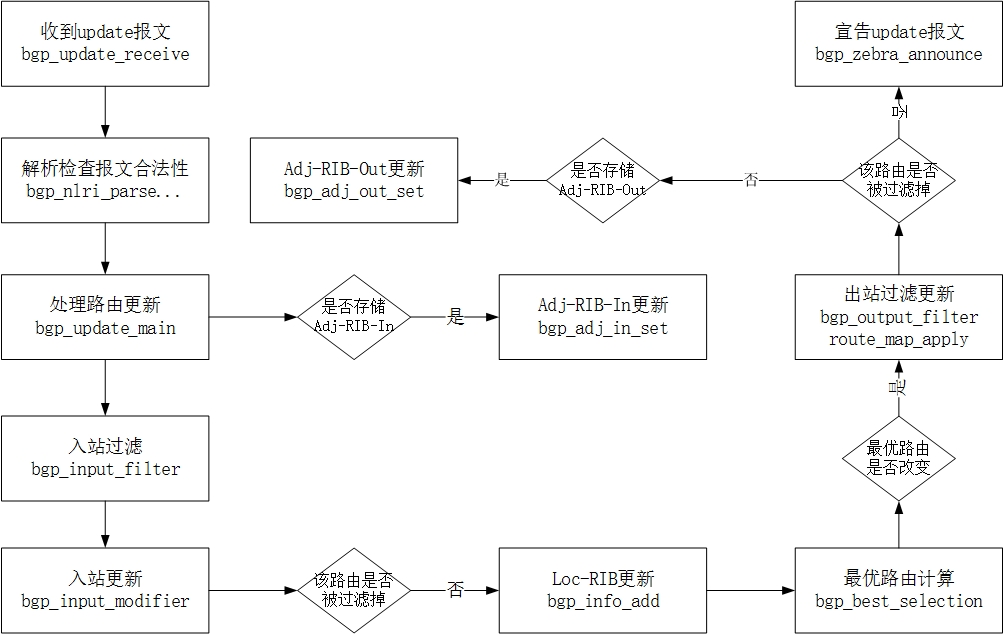
\includegraphics[width=0.8\textwidth]{route-update}
  \caption{Quagga-bgpd:BGP路由更新流程图}
  \label{fig:route-update}
\end{figure}



路由更新过程是虚拟路由器进行路由处理流程的主要部分,对应到Quagga中bgpd进程实现,路由更新的流程如图\ref{fig:route-update}:
\begin{itemize}
  \item 运行Quagga的虚拟路由器先通过bgp\_establish函数与对等体peer建立连接;
  \item 运行Quagga的虚拟路由器通过bgp\_read接收来自对等体的消息;
  \item 当收到BGP消息,通过检查头部的报文格式分析报文类型,如果是UPDATE报文,执行路由更新处理函数bgp\_update\_receive,进行UPDATE报文解析bgp\_nlri\_parse;
  \item 报文解析结束后,执行bgp\_update、bgp\_update\_main等函数进入路由更新消息的处理;
  \item 路由更新消息处理的过程中:如果需要存储Adj-RIBs-In表,进入bgp\_adj\_in\_set函数存储未经过滤的路由信息;之后执行入站过滤bgp\_input\_filter、入站更新bgp\_input\_modifier;如果更新路由没有被过滤掉,则将更新路由通过info\_make函数生成bgp\_info信息;通过bgp\_info\_add函数将bgp\_info结构体的信息加入Loc\_RIB表中,然后将其通过bgp\_process函数将该bgp\_info路由信息的处理流程加入bgp\_process\_queue队列,该队列使用先进先出的策略;
  \item 当轮到该路由信息bgp\_info处理程序时,进入bgp\_process\_main函数,执行最优路由计算bgp\_best\_selection;
  \item 如果该前缀对应的最优路由发生改变,则执行bgp\_process\_announce\_selected函数,在该函数中有出站过滤更新bgp\_announce\_check和Adj-RIBs-Out更新bgp\_adj\_out\_set;
  \item 最终通过bgp\_zebra\_announce函数将BGP路由向外宣告,且将该最优路由信息注入到RIB表中。
\end{itemize}

\subsection{路由算法}


\begin{figure}
  \centering
  % Requires \usepackage{graphicx}
  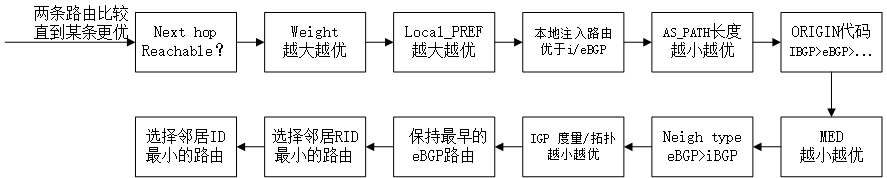
\includegraphics[width=0.9\textwidth]{route-cmp}
  \caption{Quagga-bgpd:BGP路由比较步骤}
  \label{fig:route-cmp}
\end{figure}

Quagga的bgpd进程中路由算法主要是在bgp\_best\_selection函数中实现的。针对前缀Prefix,在bgp\_table中找到该前缀对应的所有路由信息bgp\_node。路由信息的存储使用链表的数据结构,最新的路由会插在表头,所以bgp\_node存储的同一前缀的路由信息是按照更新时间由近及远进行存储。将该前缀对应的路由信息由近及远两两通过bgp\_info\_cmp进行比较,得到前缀的最优路由。两两比较选更优,比较步骤如图\ref{fig:route-cmp}。


\section{系统设计与实现}


本文提出的自治系统内的RSCP-iBGP系统的设计与实现主要涉及三大部分:自治系统内的边界路由器Route-Client路由器的设计与实现、自治系统内路由集中控制平台上Route-Server路由器的设计与实现、以及边界路由器Route-Client和路由集中控制平台Route-Server之间通信协议的设计与实现。


\subsection{边界路由器}

\begin{figure}
  \centering
  % Requires \usepackage{graphicx}
  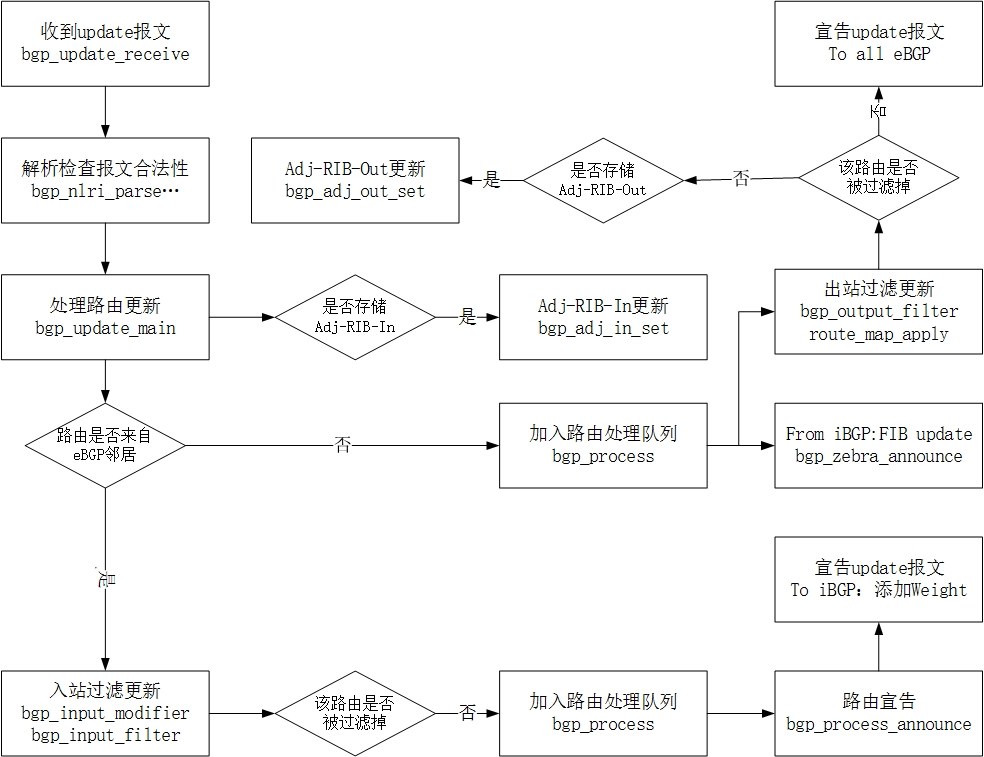
\includegraphics[width=0.9\textwidth]{rscp-route}
  \caption{RSCP-iBGP系统中边界路由器Route-Client:路由更新处理流程}
  \label{fig:rscp-route}
\end{figure}



边界路由器Route-Client收到集中平台Route-Server通过iBGP协议发来的最优路由,最优路由将会被提交到IP路由表中,相同前缀下拥有最低AD值的路由协议提交的最优路由最终会被放入IP路由表中,当路由器收到数据包时,根据IP路由表进行转发\cite{DianeTeare2016CCNP}。因为路由信息的存储和最优路由的计算均在路由控制平台上的Route-Server路由器完成,则边界路由器收到不同的路由信息(eBGP路由或者iBGP路由),需要执行不同的操作,具体的流程如图\ref{fig:rscp-route}。

当边界路由器Route-Client收到eBGP路由时,会先解析且检查该UPDATE报文的合法性,如果BGP配置文件中配置需要存储Adj-RIB-In,则将解析出来的路由信息存储到Adj-RIB-In表中。之后将该路由信息进行入站过滤和入站更新。如果该路由信息没有被eBGP的入站策略过滤掉,则将该路由加入路由处理队列等待处理。之后Route-Client会通过扩展的iBGP协议(将经过eBGP入站策略的Weight等路径属性和信息加入到UPDATE报文中),将该路由信息传输给集中平台上的Route-Server。

当边界路由器Route-Client收到iBGP路由时,会先解析且检查该UPDATE报文的合法性,如果BGP配置文件中配置需要存储Adj-RIB-Out,则将解析出来的路由信息经过出站策略后,存储到Adj-RIB-Out表中。如果该路由信息没有被eBGP的出站策略过滤掉,则将其经过出站策略的最优路由宣告给所有的eBGP邻居。



\subsection{路由集中控制平台}

RSCP-iBGP系统中的路由集中控制平台上运行的Route-Server路由器中优化了路由存储和路由计算,Route-Server路由器仅与自治系统内的边界路由器Route-Client进行iBGP连接。当Route-Server收到Route-Client发来的路由信息,Route-Server进行Loc-RIB增量存储和复式路由计算,得到自治系统内所有边界路由器的最优路由,Route-Server需要将每台边界路由器的最优路由通过扩展的iBGP协议发送到Route-Client,则Route-Server的路由宣告部分也需进行修改实现。

\subsubsection{增量路由存储}

集中控制平台上Route-Server路由器中的Loc-RIB路由存储不同于普通边界路由器的Loc-RIB路由存储。现有的自治系统内部如果有N台边界路由器,则Loc-RIB表需要存储N份。在RSCP-iBGP系统中,因为存在路由集中控制平台,则可以根据路径属性、路由比较算法等对路由信息进行增量存储。整个自治系统内的Loc-RIB均存储在路由集中控制平台Route-Server上,Route-Server上存储一张Public-Loc-RIB表,和N张iBGP邻居对应的Peer-Private-Loc-RIB表。

当收到一条UPDATE路由更新消息(Peer-info,Prefix-info, Attr-info),首先判断该路由更新是否存在于Public-Loc-RIB,如果不存在则加入Public-Loc-RIB。其次遍历每一张Peer[i]-Private-Loc-RIB表:如果表中有该Prefix且该路由信息不在Peer[i]-Private-Loc-RIB表中,则更新到对应的Peer[i]-Private-Loc-RIB;如果表中没有该Prefix,则当路由信息中的Weight属性值不为0,则仅将该更新路由更新到收到该路由信息的Route-Client边界路由器对应的Peer-Private-Loc-RIB中,同时将Public-Loc-RIB中该前缀之前的路由信息拷贝到Peer-Private-Loc-RIB,具体的实现见算法\ref{alg:incre_storage}。

\begin{algorithm}[!h]
    \caption{BGP\_INCREMENT\_STORAGE($Peer, Prefix, Attr$)}%算法标题
    \label{alg:incre_storage}
    \begin{algorithmic}[1]%一行一个标行号
        \REQUIRE
        $Peer, Prefix, Attr$
        \ENSURE
        $public\_rib, private\_ribs$
        \STATE $need\_add\_public\_rib \gets 1$
        \STATE $bgp\_info \gets make\_info(Peer, attr)$
        \IF{$(Prefix \in public\_rib) and (bgp\_info \in public\_rib[Prefix])$}
        \STATE $need\_add\_public\_rib \gets 0$
        \ENDIF
        \IF{$need\_add\_public\_rib = 1$}
        \STATE $bgp\_info\_add(bgp\_info, public\_rib[Prefix])$
        \ENDIF

        \FOR{each $Peer_i \in Established\_Peers$}
        \STATE $need\_add\_private\_rib \gets 0$

        \IF {$(Prefix \in Peer_i.private\_rib) and (bgp\_info \notin Peer_i.private\_rib[Prefix])$}
        \STATE $need\_add\_private\_rib \gets 1$
        \ENDIF
        \IF{$(Prefix \notin Peer_i.private\_rib) and (Attr.weight \ne 0) and (Peer = Peer_i)$}
        \STATE $need\_add\_private\_rib \gets 1$
        \FOR{each $(bgp\_info_i \in public\_rib[Prefix]) and (bgp\_info_i \ne bgp\_info)$}
        \STATE $bgp\_info\_add(bgp\_info_i, Peer_i.private\_rib[Prefix])$
        \ENDFOR
        \ENDIF

        \IF{$need\_add\_private\_rib = 1$}
        \STATE $bgp\_info\_add(bgp\_info, Peer_i.private\_rib[Prefix])$
        \ENDIF

        \ENDFOR
    \end{algorithmic}
\end{algorithm}


\subsubsection{复式路由计算}


在本文提出的RSCP-iBGP系统中的增量路由存储模块,路由计算结果与Weight路由属性相关的Prefix路由单独存储到Private\_Loc\_RIB,不受Weight路由属性影响的Prefix路由仅存储一份于Public\_Loc\_RIB。复式路由计算结合增量路由存储,与Weight相关的Peer的Prefix最优路由根据Peer的Private\_Loc\_RIB单独进行计算,其余的与Weight无关的Peer的Prefix最优路由通过Public\_Loc\_RIB进行计算。

当集中平台收到一条Prefix的路由信息时,需要计算出自治系统内所有边界路由器的该Prefix的最优路由。先通过Public\_Loc\_RIB表计算出所有Peer的最优路由,之后遍历所有对等体的Private\_Loc\_RIB,如果某个$Peer_i$的Private\_Loc\_RIB存储该Prefix的路由信息,则该$Peer_i$的Prefix最优路由更新为$Peer_i$的Private\_Loc\_RIB计算出的最优路由,具体实现见算法\ref{alg:multi_routing_calculation}。

\begin{algorithm}[htb]
    \caption{BGP\_Multi\_Routing\_Calculation($Peers, Prefix, public\_rib$)}%算法标题
    \label{alg:multi_routing_calculation}
    \begin{algorithmic}[1]%一行一个标行号
        \REQUIRE
        $Established\_Peers[1...j], Prefix, public\_rib$
        \ENSURE
        $Peer\_BestRoutes[1...j]$
        \STATE $Peer\_BestRoutes[1...j] \gets  bgp\_pub\_best\_selection(Prefix, public\_rib)$
        \FOR{each $Peer_i \in Established\_Peers[1...j]$}
        \IF {$(Prefix \in Peer_i.private\_rib)$}
        \STATE $Peer\_BestRoutes[i] \gets  bgp\_pri\_best\_selection(Prefix, Peer_i.private\_rib)$
        \ENDIF
        \ENDFOR
        \RETURN $Peer\_BestRoutes[1...j]$
    \end{algorithmic}
\end{algorithm}

通过路由集中控制平台Route-Server中存储的Public\_Loc\_RIB表,计算出与Weight无关的所有Peer针对Prefix的最优路由。使用Public\_Loc\_RIB计算所有边界路由器最优路由的过程,主要分为两大部分:
\begin{itemize}
  \item 各边界路由器的衡量标准相同,依次执行删除Prefix对应的路由集合中非最高本地优先级、非最短As-path、相同AS非最低MED值等3个操作,在每个操作之后判断该Prefix对应的路由集合中是否仅剩一条路由,如果仅剩一条路由,则为所有边界路由器的该Prefix的最优路由,具体实现见算法\ref{alg:public_selection_one};
  \item 因为边界路由器之间的IGPcost各有不同,所以如果在各边界路由器衡量标准相同的筛选条件下没有计算出最优路由,则之后自治系统内的每台边界路由器的最优路由需要单独进行计算,基于Prefix对应的路由集合依次执行删除非最短IGPcost的路由、非最早eBGP路由、非最小的接收该路由的eBGP邻居route-id(存储在路由集中平台)、非最小的接收该路由的eBGP邻居IP地址(存储在路由集中平台)等操作,在每个操作之后判断该Prefix对应的路由集合中是否仅剩一条路由,如果仅剩一条路由,则为该边界路由器对应的该Prefix的最优路由,具体实现见算法\ref{alg:public selection_two}。\\
\end{itemize}


与Weight相关的Peer的Prefix最优路由,需要根据Peer的Private\_Loc\_RIB表中的Prefix的全部路由进行单独计算。通过将Peer的Private\_Loc\_RIB表中的Prefix的全部路由放入路由集合,依次执行删除路由集合中的非最大Weight值、非最高本地优先级、非最短As-path、相同AS非最低MED值、非最短IGPcost的路由、非最早eBGP路由、非最小的接收该路由的eBGP邻居route-id(存储在路由集中平台)、非最小的接收该路由的eBGP邻居IP地址(存储在路由集中平台)等操作。在每个操作之后判断该Prefix对应的路由集合中是否仅剩一条路由,如果仅剩一条路由,则为该边界路由器对应的该Prefix的最优路由。

\begin{algorithm}[!h]
    \caption{bgp\_pub\_best\_selection($Prefix, public\_rib, Established\_Peers$)}
    \label{alg:public_selection_one}
    \begin{algorithmic}[1]%一行一个标行号
        \REQUIRE
        $Prefix, public\_rib, Established\_Peers[1...j]$
        \ENSURE
        $Peer\_BestRoutes[1...j]$
        \STATE $Public\_BestRoute \gets NULL$
        \STATE $public\_rib\_t \gets public\_rib$
        \STATE $public\_rib\_t \gets delete\_nonMaxLocPref(public\_rib\_t)$
        \IF {$public\_rib\_t.size = 1$}
        \STATE $Public\_BestRoute  \gets public\_rib\_t[0]$
        \ENDIF

        \STATE $public\_rib\_t \gets delete\_nonMinAsPathLength(public\_rib\_t)$
        \IF {$public\_rib\_t.size = 1$}
        \STATE $Public\_BestRoute  \gets public\_rib\_t[0]$
        \ENDIF

        \STATE $public\_rib\_t \gets delete\_nonMinMedSameAs(public\_rib\_t)$
        \IF {$public\_rib\_t.size = 1$}
        \STATE $Public\_BestRoute  \gets public\_rib\_t[0]$
        \ENDIF

        \IF {$Peer\_BestRoutes \ne NULL$}
        \FOR{each $Peer\_BestRoutes[i] \in Peer\_BestRoutes[1...j]$}
        \STATE $Peer\_BestRoutes[i] \gets Public\_BestRoute $
        \ENDFOR
        \STATE \textbf{return} $Peer\_BestRoutes[1...j]$
        \ENDIF

        \FOR{each $Peer_i \in Established\_Peers[1...j]$}
        \STATE $Peer\_BestRoutes[i] \gets get\_specialBestRoute\_fromPublicRib(peer_i,public\_rib\_t)$
        \ENDFOR
        \STATE \textbf{return} $Peer\_BestRoutes[1...j]$
    \end{algorithmic}
\end{algorithm}





\subsubsection{路由宣告}
当自治系统内的路由集中控制平台上运行的Route-Server路由器,收到自治系统内的边界路由器Route-Client发来的iBGP路由,Route-Server对该iBGP路由信息进行解析(包括从UPDATE报文中解析Weight路径属性),之后Router-Server会根据存储的路由表项计算出该路由前缀的针对自治系统内所有边界路由器的最优路由,最后将对应的最优路由宣告给对应的边界路由器(如果边界路由器Route-Client-i的最优路由是该边界路由器自身Route-Client-i收到的,next-hop设置为对应的直连eBGP邻居;如果边界路由器Route-Client-i的最优路由是其他边界路由器Route-Client-j从eBGP邻居收到的,next-hop设置为Route-Client-j的与Route-Client-i一个网段的地址)。

在路由宣告的过程中,Route-Server上运行的软件路由器会检测宣告路由的合法性,因为Quagga版本中判断路由器是否为路由反射器的标准为该路由信息是否从iBGP邻居接收并宣告给iBGP邻居,所以在Route-Server上运行的软件路由器代码需要在接收路由后或者宣告路由前,对路由反射器的检测代码进行修改。

传统的路由信息传输到路由器之后,路由器会检测其Next-hop值是否可达,则一般会通过在BGP的配置文件中给iBGP邻居设置Next-hop-self属性,保证Next-hop可达性。在本文提出的RSCP-iBGP系统中,需要在集中控制平台上进行最优路由的计算,并将最后的计算结果通过iBGP协议传输给边界路由器Route-Client,则需要将eBGP邻居的Next-hop值传输到集中平台,则不设置Next-hop-self属性,Route-Client边界路由器会将eBGP邻居的Next-hop值传到集中平台,且在集中平台上暂时不做可达性检测。未来可将Route-Client的eBGP可达邻居信息进行实时管理更新。基于集中平台上管理的自治系统内部的Route-Client的eBGP可达邻居信息,可在集中平台Route-Server上判断路由从eBGP邻居过来的Next-hop的可达性,从而确保路由信息的有效性。

\begin{algorithm}[!h]
    \caption{get\_specialBestRoute\_fromPublicRib($peer,public\_rib$)}
    \label{alg:public selection_two}
    \begin{algorithmic}[1]%一行一个标行号
         \REQUIRE
        $peer,public\_rib$
        \ENSURE
        $Peer\_BestRoute$
        \STATE $public\_rib\_t \gets public\_rib$
        \STATE $public\_rib\_t \gets delete\_nonMinIGPcost(peer, public\_rib\_t)$
        \IF {$public\_rib\_t.size = 1$}
        \STATE \textbf{return} $public\_rib\_t[0]$
        \ENDIF
        \STATE $public\_rib\_t \gets delete\_nonEarliestRoute(peer, public\_rib\_t)$
        \IF {$public\_rib\_t.size = 1$}
        \STATE \textbf{return} $public\_rib\_t[0]$
        \ENDIF
        \STATE $public\_rib\_t \gets delete\_nonMinEbgpPeer\_Route-id(peer, public\_rib\_t)$
        \IF {$public\_rib\_t.size = 1$}
        \STATE \textbf{return} $public\_rib\_t[0]$
        \ENDIF
        \STATE $public\_rib\_t \gets delete\_nonMinEbgpPeer\_IPAddr(peer, public\_rib\_t)$
        \IF {$public\_rib\_t.size = 1$}
        \STATE \textbf{return} $public\_rib\_t[0]$
        \ENDIF
        \STATE \textbf{return} $public\_rib\_t[0]$
    \end{algorithmic}
\end{algorithm}


\subsection{通信接口}
通信接口通过扩展的iBGP协议进行实现,边界路由器Route-Client需要发送携带Weight路径属性的UPDATE报文信息到集中平台Route-Server,且Route-Server收到扩展iBGP协议发来的携带Weight路径属性的UPDATE报文需要能够进行正常识别和解析。

边界路由器上运行的BGP协议需要在给iBGP邻居发送UPDATE报文的时候携带Weight路径属性,所以在边界路由器上运行的软件路由器Quagga中,需要修改UPDATE报文的Path Attributes部分,增加传输Weight路径属性。在Quagga中的BGP协议代码实现UPDATE报文封装的过程中,Path Attributes的组包实现函数为bgp\_packet\_attribute(bgpd\_attr.c文件中),在其他属性添加结束后,在字节流后添加Path Attribute的三元组,具体的实现见算法\ref{alg:add_weight}。传输Weight属性的三元组中,Flag=0x40和Type Code=0x1f,Length=0x02,Value值长度为2个字节。如果传输的Weight值为150,则对应的传输Weight的Path  Attribute为0x401f020096。

\begin{algorithm}[!h]
    \caption{BGP\_PACKET\_ATTRIBUTE($peer,attr,stream...$)}%算法标题
    \label{alg:add_weight}
    \begin{algorithmic}[1]%一行一个标行号
        \STATE $stream \gets Path\_Attributes\_Except\_Weight\_Info$
        \IF{$peer->sort = BGP\_PEER\_IBGP$}
        \STATE $stream \gets stream+BGP\_ATTR\_FLAG\_TRANS$
        \STATE $stream \gets stream+BGP\_ATTR\_WEIGHT\_TYPE\_CODE$
        \STATE $stream \gets stream+BGP\_ATTR\_WEIGHT\_LENGTH$
        \STATE $stream \gets stream+BGP\_ATTR\_WEIGHT\_VALUE$
        \ENDIF
    \end{algorithmic}
\end{algorithm}


集中平台上Route-Server收到携带Weight路径属性值的UPDATE报文后,需要对其进行正确的解析。Quagga中的BGP协议代码实现Path Attributes解析的函数为bgp\_attr\_parse(bgpd\_attr.c文件中),根据Type Code执行不同的Path Attribute解析函数,Weight属性的解析函数需要检查Length是否为2。如果不为2,需要执行bgp\_notify\_send函数,回复对等体NOTIFICATION报错(Path Attribute长度错误)。



\section{本章小结}
本章对RSCP-iBGP系统的实现平台Quagga进行了详细的介绍,了解虚拟路由器Quagga的BGP路由实现之后,针对RSCP-iBGP系统的需求,具体描述了RSCP-iBGP系统中边界路由器、集中控制平台,通信协议的设计与实现。
